%%
%% This is file `sample-manuscript.tex',
%% generated with the docstrip utility.
%%
%% The original source files were:
%%
%% samples.dtx  (with options: `all,proceedings,bibtex,manuscript')
%% 
%% IMPORTANT NOTICE:
%% 
%% For the copyright see the source file.
%% 
%% Any modified versions of this file must be renamed
%% with new filenames distinct from sample-manuscript.tex.
%% 
%% For distribution of the original source see the terms
%% for copying and modification in the file samples.dtx.
%% 
%% This generated file may be distributed as long as the
%% original source files, as listed above, are part of the
%% same distribution. (The sources need not necessarily be
%% in the same archive or directory.)
%%
%%
%% Commands for TeXCount
%TC:macro \cite [option:text,text]
%TC:macro \citep [option:text,text]
%TC:macro \citet [option:text,text]
%TC:envir table 0 1
%TC:envir table* 0 1
%TC:envir tabular [ignore] word
%TC:envir displaymath 0 word
%TC:envir math 0 word
%TC:envir comment 0 0
%%
%% The first command in your LaTeX source must be the \documentclass
%% command.
%%
%% For submission and review of your manuscript please change the
%% command to \documentclass[manuscript, screen, review]{acmart}.
%%
%% When submitting camera ready or to TAPS, please change the command
%% to \documentclass[sigconf]{acmart} or whichever template is required
%% for your publication.
%%
%%
\documentclass[manuscript,screen,review]{acmart}
%%
%% \BibTeX command to typeset BibTeX logo in the docs
\AtBeginDocument{%
  \providecommand\BibTeX{{%
    Bib\TeX}}}

%% Rights management information.  This information is sent to you
%% when you complete the rights form.  These commands have SAMPLE
%% values in them; it is your responsibility as an author to replace
%% the commands and values with those provided to you when you
%% complete the rights form.
\setcopyright{acmlicensed}
\copyrightyear{2018}
\acmYear{2018}
\acmDOI{XXXXXXX.XXXXXXX}
%% These commands are for a PROCEEDINGS abstract or paper.
\acmConference[Konferenz Akronym {'XX]Vergewissern Sie sich, den korrekten Konferenztitel von Ihrer Rechtebestätigung zu geben {emailWoodstock, NY}}
{Juni 03–05, 2018}%%
%%  Uncomment \acmBooktitle if the title of the proceedings is different
%%  from ``Proceedings of ...''!
%%
%%\acmBooktitle{Woodstock '18: ACM Symposium on Neural Gaze Detection,
%%  June 03--05, 2018, Woodstock, NY}
\acmISBN{978-1-4503-XXXX-X/2018/06}

%%
%% Submission ID.
%% Use this when submitting an article to a sponsored event. You'll
%% receive a unique submission ID from the organizers
%% of the event, and this ID should be used as the parameter to this command.
%%\acmSubmissionID{123-A56-BU3}

%%
%% For managing citations, it is recommended to use bibliography
%% files in BibTeX format.
%%
%% You can then either use BibTeX with the ACM-Reference-Format style,
%% or BibLaTeX with the acmnumeric or acmauthoryear sytles, that include
%% support for advanced citation of software artefact from the
%% biblatex-software package, also separately available on CTAN.
%%
%% Look at the sample-*-biblatex.tex files for templates showcasing
%% the biblatex styles.
%%

%%
%% The majority of ACM publications use numbered citations and
%% references.  The command \citestyle{authoryear} switches to the
%% "author year" style.
%%
%% If you are preparing content for an event
%% sponsored by ACM SIGGRAPH, you must use the "author year" style of
%% citations and references.
%% Uncommenting
%% the next command will enable that style.
%%\citestyle{acmauthoryear}

%%
%% end of the preamble, start of the body of the document source.
\begin{document}

%%
%% The "title" command has an optional parameter,
%% allowing the author to define a "short title" to be used in page headers.
\title{Der Name des Titels ist Hoffnung}

%%
%% The "author" command and its associated commands are used to define
%% the authors and their affiliations.
%% Of note is the shared affiliation of the first two authors, and the
%% "authornote" and "authornotemark" commands
%% used to denote shared contribution to the research.

\authornote{Both authors contributed equally to this research.} \email{trovato@corporation.com} \orcid{1234-5678-9012}

\authornotemark[1] \email{webmaster@marysville-ohio.com} \affiliation{%
  \institution{Institute for Clarity in Documentation}
  \city{Dublin}
  \state{Ohio}
  \country{USA}
}

\affiliation{%
  \institution{The Th{\o}rväld Group}
  \city{Hekla}
  \country{Iceland}} \email{larst@affiliation.org}

\affiliation{%
  \institution{Inria Paris-Rocquencourt}
  \city{Rocquencourt}
  \country{France}
}

\affiliation{%
 \institution{Rajiv Gandhi University}
 \city{Doimukh}
 \state{Arunachal Pradesh}
 \country{India}}

\affiliation{%
  \institution{Tsinghua University}
  \city{Haidian Qu}
  \state{Beijing Shi}
  \country{China}}

\affiliation{%
  \institution{Palmer Research Laboratories}
  \city{San Antonio}
  \state{Texas}
  \country{USA}} \email{cpalmer@prl.com}

\affiliation{%
  \institution{The Th{\o}rväld Group}
  \city{Hekla}
  \country{Iceland}} \email{jsmith@affiliation.org}

\affiliation{%
  \institution{The Kumquat Consortium}
  \city{New York}
  \country{USA}} \email{jpkumquat@consortium.net}

%%
%% By default, the full list of authors will be used in the page
%% headers. Often, this list is too long, and will overlap
%% other information printed in the page headers. This command allows
%% the author to define a more concise list
%% of authors' names for this purpose.
\renewcommand{\shortauthors}{Trovato et al.}

%%
%% The abstract is a short summary of the work to be presented in the
%% article.
\begin{abstract}
  Ein klares und gut dokumentiertes \LaTeX-Dokument wird als ein Artikel präsentiert, der von ACM in einer Konferenz- oder Zeitschriftenpublikation formatiert wird. Basierend auf der Dokument-Klasse "Acmart" präsentiert und erklärt dieser Artikel viele der gängigen Variationen sowie viele der Formatierungselemente, die ein Autor bei der Erstellung der Dokumentation seiner Arbeit verwenden kann.
\end{abstract}

%%
%% The code below is generated by the tool at http://dl.acm.org/ccs.cfm.
%% Please copy and paste the code instead of the example below.
%%
\begin{CCSXML}
<ccs2012> <concept_id>00000.0000.0000.00000000 </concept_id> <concept_desc>Verwenden Sie diesen Code nicht, erzeugen Sie die korrekten Bedingungen für Ihr Papier </concept_desc> <concept_significance>500</concept_significance> <concept> <concept_id>00000.0000000000000 </concept_desc> <concept_desc>Verwenden Sie diesen Code nicht, erzeugen Sie die korrekten Bedingungen für Ihr Papier </concept_desc> <concept_significance>300</concept_significance> <concept> <concept_id>00000000.000000000000000000 </concept_id> <concept_desc>Verwenden Sie diesen Code nicht, erzeugen Sie die korrekten Bedingungen für Ihr Papier </concept_desc> <concept_desc> <concept_significance> <100 <concept_signific> </concept_concept_design>
\end{CCSXML}

\ccsdesc[500] \ccsdesc[300] \ccsdesc{Do Not Use This Code~Generate the Correct Terms for Your Paper} \ccsdesc[100]

{Verwenden Sie diesen Code nicht Erzeugen Sie die richtigen Bedingungen für Ihr Papier}{Verwenden Sie diesen Code nicht Erzeugen Sie die richtigen Bedingungen für Ihr Papier}{Verwenden Sie diesen Code nicht Erzeugen Sie die richtigen Bedingungen für Ihr Papier}%%
%% Keywords. The author(s) should pick words that accurately describe
%% the work being presented. Separate the keywords with commas.
\keywords{Do, Not, Use, This, Code, Put, the, Correct, Terms, for,
  Your, Paper}

\received{20 February 2007} {\received[überarbeitet]12. März 2009} {\received[angenommen]5. Juni 2009}

%%
%% This command processes the author and affiliation and title
%% information and builds the first part of the formatted document.
\maketitle

\section{Einleitung}
Die im Jahr 2017 eingeführte konsolidierte Artikelvorlage von ACM bietet einen konsistenten \LaTeX-Stil für die Verwendung in ACM-Publikationen und beinhaltet die für zukünftige Bemühungen der Digital Library notwendige Barrierefreiheit und Metadaten-Extraktionsfunktionalität. Zahlreiche ACM- und SIG-spezifische \LaTeX-Vorlagen wurden untersucht und ihre einzigartigen Funktionen wurden in diese einzige neue Vorlage integriert.

Wenn Sie neu in der Veröffentlichung mit ACM sind, ist dieses Dokument ein wertvoller Leitfaden für den Prozess der Vorbereitung Ihrer Arbeit für die Veröffentlichung. Wenn Sie bereits mit ACM veröffentlicht haben, bietet dieses Dokument Einblick und Anleitung in neuere Änderungen an der Artikelvorlage.

Die Dokument-Klasse kann verwendet werden, um Artikel für jede ACM-Publikation vorzubereiten — Konferenz oder Zeitschrift, und für jede Phase der Veröffentlichung, von der Überprüfung bis zur endgültigen   .camera-ready-ready-Kopie, um die eigene Version des Autors, mit wenigen Änderungen an der Quelle.

{\itshape sehr}\section{Vorlage im Überblick}
Wie bereits in der Einleitung erwähnt, kann die Dokument-Klasse von SIGGRAPH verwendet werden, um viele verschiedene Arten von Dokumentation vorzubereiten — eine doppelanonyme erste Vorlage eines umfassenden technischen Papiers, ein zweiseitiges SIGGRAPH Emerging Technologies-Abstract, ein camera-ready-ready-Zeitschriftartikel, ein SIGCHI Extended Abstract und vieles mehr — alles durch Auswahl der entsprechenden und .

Dieses Dokument erklärt die Hauptmerkmale der Dokumentklasse. Für weitere Informationen steht das Dokument unter \url{https://www.acm.org/publications/proceedings-template} zur Verfügung.

{\itshape Vorlagestil}{\itshape Vorlagenparameter}{\itshape \LaTeX Benutzerhandbuch}\subsection{Vorlagenstile}

Der primäre Parameter, der der Dokument-Klasse ""\verb|acmart|" gegeben wird, entspricht der Art der Publikation oder der SIG-Veröffentlichung des Werkes. Dieser Parameter ist in eckigen Klammern eingeschlossen und ist Teil des Befehls:
{\itshape Vorlagestil}{\verb|documentclass|}\begin{verbatim}
  \documentclass[STYLE]{acmart}
\end{verbatim}

Zeitschriften verwenden einen von drei Vorlagenstilen. Alle bis auf drei ACM-Zeitschriften verwenden den Vorlagenstil:
{\verb|acmsmall|}\begin{itemize}
\item {\texttt{acmsmall}}: Der Standard-Template-Stil des Journals.
\item {\texttt{acmlarge}}: Verwendet von JOCCH und TAP.
\item {\texttt{acmtog}}: Verwendet von TOG.
\end{itemize}

Der Großteil der Dokumentation des Konferenzprozesses wird den Template-Stil verwenden.
{\verb|acmconf|}\begin{itemize}
\item {\texttt{sigconf}}: Der Stil der Standard-Procedure-Vorlage.
\item{\texttt{sigchi}}: Wird für SIGCHI-Konferenzartikel verwendet.
\item{\texttt{sigplan}}: Wird für SIGPLAN-Konferenzartikel verwendet.
\end{itemize}

\subsection{Vorlagenparameter}

Neben der Angabe der für die Formatierung Ihrer Arbeit zu verwenden, gibt es eine Reihe von denen ändern einen Teil der angewandten Vorlage Stil. Eine vollständige Liste dieser Parameter finden Sie in der

Häufig verwendete Parameter oder Kombinationen von Parametern umfassen:
{\itshape Vorlagestil}{\itshape Vorlagenparameter}{\itshape \LaTeX Benutzerhandbuch.}\begin{itemize}
\item {\texttt{anonymous,review}}: Geeignet für eine Doppelanonymisierung. Anonymisiert die Arbeit und enthält Zeilennummern. Verwenden Sie mit dem Befehl \texttt{\string\acmSubmissionID}, um die eindeutige ID der Einreichung auf jeder Seite des Werkes zu drucken.
\item{\texttt{authorversion}}: Produziert eine Version des Werkes geeignet für die Entsendung durch den Autor.
\item{\texttt{screen}}: Erzeugt farbige Hyperlinks.
\end{itemize}

Dieses Dokument verwendet den folgenden String als ersten Befehl in der Quelldatei:
\begin{verbatim}
\documentclass[manuscript,screen,review]{acmart}
\end{verbatim}

\section{Änderungen}

Die Änderung der Vorlage — einschließlich, aber nicht beschränkt auf: Einstellen von Rändern, Schriftgrößen, Zeilenabstand, Absatz- und Listendefinitionen und die Verwendung des Befehls \verb|\vspace| zur manuellen Einstellung des vertikalen Abstands zwischen den Elementen Ihrer Arbeit — ist nicht gestattet.



{\bfseries Ihr Dokument wird Ihnen zur Revision zurückgegeben, wenn Änderungen entdeckt werden.}\section{Schriftarten}

Für die Dokument-Klasse "[\verb|acmart|]" ist die Verwendung der Schrift-Familie "Libertine" erforderlich. Ihre Installation "\TeX" sollte diesen Satz von Paketen enthalten. Bitte ersetzen Sie keine anderen Schriftarten. Die Pakete "\verb|lmodern|" und "\verb|ltimes|" sollten nicht verwendet werden, da sie die eingebauten Schrift-Familien überschreiben.

\section{Titelinformation}

Der Titel Ihrer Arbeit sollte Großbuchstaben entsprechend verwenden - \url{https://capitalizemytitle.com/} hat nützliche Regeln für die Kapitalisierung. Verwenden Sie den Befehl, um den Titel Ihrer Arbeit zu definieren. Wenn Ihre Arbeit einen Untertitel hat, definieren Sie ihn mit dem Befehl. Fügen Sie Zeilenumbrüche nicht in Ihren Titel ein.

Wenn Ihr Titel lang ist, müssen Sie eine kurze Version definieren, die in den Seitenkopfzeilen verwendet werden soll, um überlappenden Text zu verhindern.
{\verb|title|}{\verb|subtitle|}\begin{verbatim}
  \title[short title]{full title}
\end{verbatim}

\section{Autoren und Mitgliedschaften}

Jeder Autor muss separat für die genaue Metadaten-Identifikation definiert werden. Ausnahmsweise können mehrere Autoren eine Zugehörigkeit teilen. Autorennamen sollten nicht abgekürzt werden; volle Vornamen verwenden, wo immer möglich. E-Mail-Adressen von Autoren einbeziehen, wann immer möglich.

Eine Gruppierung von Autorennamen oder E-Mail-Adressen oder die Bereitstellung eines Alias der E-Mail-Adressen, wie unten gezeigt, ist nicht akzeptabel:
\begin{verbatim}
  \author{Brooke Aster, David Mehldau}
  \email{dave,judy,steve@university.edu}
  \email{firstname.lastname@phillips.org}
\end{verbatim}

Die Befehle \verb|authornote| und \verb|authornotemark| erlauben es, eine Notiz für mehrere Autoren zu verwenden – zum Beispiel, wenn die ersten beiden Autoren eines Artikels in gleicher Weise zur Arbeit beigetragen haben.

Wenn Ihre Autorenliste lang ist, müssen Sie eine verkürzte Version der Autorenliste definieren, die in den Seitenkopfzeilen verwendet werden soll, um Überschneidungen zu vermeiden. Der folgende Befehl sollte kurz nach der letzten \verb|\author{}| Definition gesetzt werden:
\begin{verbatim}
  \renewcommand{\shortauthors}{McCartney, et al.}
\end{verbatim}
Durch das Weglassen dieses Befehls wird die Verwendung einer verketteten Liste aller Autorennamen erzwungen, was zu Überschneidungen von Texten in den Seitenkopfzeilen führen kann.

Die Dokumentation der Artikelvorlage, die unter \url{https://www.acm.org/publications/proceedings-template} verfügbar ist, enthält eine vollständige Erklärung dieser Befehle und Tipps für ihre effektive Verwendung.

Beachten Sie, dass die Adressen der Autoren für Zeitschriftenartikel verbindlich sind.

\section{Rechte Information}

Die Autoren jeder von ACM veröffentlichten Arbeit müssen ein Rechtsformular ausfüllen. Je nach Art der Arbeit und der Wahl der Rechteverwaltung durch den Autor kann dies eine Urheberrechtsübertragung, Erlaubnis, Lizenz oder eine OA (Open Access) Vereinbarung sein.

Unabhängig von der Wahl der Rechteverwaltung erhält der Autor eine Kopie des ausgefüllten Rechtsformulars, sobald es eingereicht wurde. Dieses Formular enthält \LaTeX Befehle, die in das Quelldokument kopiert werden müssen. Wenn die Dokumentenquelle kompiliert wird, fügen diese Befehle und ihre Parameter formatierten Text zu mehreren Bereichen des endgültigen Dokuments hinzu:
\begin{itemize}
\item der Text des Referenzformats auf der ersten Seite.
\item der Text auf der ersten Seite.
\item die Konferenzinformationen in der (den) Seitenkopf(en).
\end{itemize}

Rechte Informationen sind einzigartig für die Arbeit; wenn Sie mehrere Werke für ein Ereignis vorbereiten, stellen Sie sicher, dass Sie den richtigen Satz von Befehlen mit jedem der Werke verwenden.

Der ACM-Referenzformat-Text ist für alle Artikel über eine Seite in der Länge erforderlich und ist optional für einseitige Artikel (Abstracts).

\section{CCS-Konzepte und benutzerdefinierte Schlüsselwörter}

Zwei Elemente der Dokument-Klasse bieten leistungsstarke taxonomische Tools für Sie, um Lesern zu helfen, Ihre Arbeit in einer Online-Suche zu finden.

Das ACM Computing Classification System — \url{https://www.acm.org/publications/class-2012} — ist ein Satz von Klassifikatoren und Konzepten, die die Rechendisziplin beschreiben. Autoren können Einträge aus diesem Klassifikationssystem über \url{https://dl.acm.org/ccs/ccs.cfm} auswählen und die Befehle generieren, die in die \LaTeX-Quelle aufgenommen werden sollen.

Benutzerdefinierte Schlüsselwörter sind eine durch Komma getrennte Liste von Wörtern und Sätzen der Autoren, die eine flexiblere Art und Weise bieten, die vorgestellte Forschung zu beschreiben.

CCS-Konzepte und benutzerdefinierte Keywords sind für alle Artikel über zwei Seiten Länge erforderlich und optional für ein- und zweiseitige Artikel (oder Abstracts).

\section{Trennbefehle}

Ihre Arbeit sollte Standard \LaTeX-Sektionsbefehle verwenden: \verb|\section|, \verb|\subsection|, \verb|\subsubsection|, \verb|\paragraph| und \verb|\subparagraph|. Die Sektionsebenen bis \verb|\subsusection| sollten nummeriert werden; entfernen Sie die Nummerierung nicht von den Befehlen.

Simulieren eines Abschnittsbefehls, indem Sie das erste Wort oder die ersten Worte eines Absatzes in Fettdruck oder kursiver Text setzen

Nachfolgend finden Sie Beispiele für Trennbefehle.

{\bfseries nicht erlaubt.}\subsection{Unterabschnitt}
\label{sec:subsection}

Das ist ein Unterabschnitt.

§§§ Unterabschnitt

\label{sec:subsubsection}

Dies ist ein Unterabschnitt.

\paragraph{Absatz}

Das ist ein Absatz.

Unterabsatz

Dies ist ein Unterabsatz.

\section{Tabellen}

Die Dokument-Klasse enthält das Paket \url{https://ctan.org/pkg/booktabs}, um qualitativ hochwertige Tabellen zu erstellen.

Die Tabellenbezeichnungen werden auf den Tisch gelegt.

Da Tabellen nicht auf Seiten aufgeteilt werden können, ist die beste Platzierung für sie in der Regel die oberste der Seite am nächsten ihrer ursprünglichen Anführung. Um sicherzustellen, dass diese richtige     . floating" Platzierung von Tabellen, verwenden Sie die \textbf{Umgebungstabelle}, um den Inhalt des Tabellens und die Tabellenbezeichnung schließen. Der Inhalt des Tabellens selbst muss in der \textbf{tabellarischen} Umgebung gehen, um richtig in Zeilen und Spalten ausgerichtet werden, mit den gewünschten horizontalen und vertikalen Regeln. Wieder, detaillierte Anweisungen auf \textbf{tabellarischen} Material finden Sie in \textit{der \LaTeX Benutzerhandbuch}.

Unmittelbar nach diesem Satz folgt der Punkt, an dem Tabelle \ref{tab:freq} in der Eingabedatei enthalten ist; vergleicht die Platzierung der Tabelle hier mit der Tabelle in der gedruckten Ausgabe dieses Dokuments.

{Nr. 1_ oben}\begin{table}
  \caption{Häufigkeit von Sonderzeichen}
  \label{tab:freq}
  \begin{tabular}{ccl}
    \toprule
    Non-English or Math&Frequency&Comments\\
    \midrule
    \O & 1 in 1,000& For Swedish names\\
    $\pi$ & 1 in 5& Common in math\\
    \$ & 4 in 5 & Used in business\\
    $\Psi^2_1$ & 1 in 40,000& Unexplained usage\\
  \bottomrule
\end{tabular}
\end{table}

Um eine breitere Tabelle zu setzen, die die gesamte Breite des Live-Bereichs der Seite aufnimmt, verwenden Sie die \textbf{Environment-Tabelle}*, um den Inhalt der Tabelle und die Tabellenbezeichnung zu umschließen. Wie bei einer einspaltigen Tabelle wird diese breite Tabelle an einen für wünschenswerter gehaltenen Ort gelangen. Unmittelbar nach diesem Satz folgt der Punkt, an dem Tabelle \ref{tab:commands} in der Eingabedatei enthalten ist; wiederum ist es lehrreich, die Platzierung der Tabelle hier mit der Tabelle in der gedruckten Ausgabe dieses Dokuments zu vergleichen.

\begin{table*}
  \caption{Einige typische Befehle}
  \label{tab:commands}
  \begin{tabular}{ccl}
    \toprule
    Command &A Number & Comments\\
    \midrule
    \texttt{{\char'134}author} & 100& Author \\
    \texttt{{\char'134}table}& 300 & For tables\\
    \texttt{{\char'134}table*}& 400& For wider tables\\
    \bottomrule
  \end{tabular}
\end{table*}

Verwenden Sie immer Midrule, um Tabellenkopfzeilen von Datenzeilen zu trennen und sie nur für diesen Zweck zu verwenden. Dies ermöglicht es assistiven Technologien, Tabellenkopfzeilen zu erkennen und ihre Benutzer leichter beim Navigieren von Tabellen zu unterstützen.

\section{Mathematische Gleichungen}
Sie können mathematische Gleichungen in drei verschiedenen Stilen anzeigen: Inline-, nummerierte oder nicht-nummerierte Anzeige. Jede der drei werden in den nächsten Abschnitten diskutiert.

\subsection{Inline (In-Text) Gleichungen}
Eine Formel, die im laufenden Text erscheint, wird als Inline- oder Intext-Formel bezeichnet. Sie wird von der \textbf{mathematischen} Umgebung erzeugt, die mit der üblichen \texttt{{\char'134}begin\,\ldots{\char'134}end}-Konstruktion oder mit der kurzen Form \texttt{\$\,\ldots\$} aufgerufen werden kann. Sie können jedes der Symbole und Strukturen verwenden, von $\alpha$ bis $\omega$, verfügbar in \LaTeX \cite{Lamport:LaTeX}; dieser Abschnitt zeigt einfach einige Beispiele von Intext-Gleichungen im Kontext. Beachten Sie, wie diese Gleichung:
\begin{math}
  Lim_x=0
{n→ ∧}\end{math}, hier im In-Line-Mathematik-Stil gesetzt, sieht etwas anders aus, wenn es im Display-Stil gesetzt wird. (Siehe nächster Abschnitt).

\subsection{Gleichungen anzeigen}
Eine nummerierte Displaygleichung – eine durch den vertikalen Raum aus dem Text gesetzte und horizontal zentrierte – wird durch die \textbf{Gleichungsumgebung} erzeugt. Eine nummerierte Displaygleichung wird durch die \textbf{Displaymath-Umgebung} erzeugt.

Auch in beiden Umgebungen können Sie jedes der Symbole und Strukturen verwenden, die in \LaTeX\@ verfügbar sind; dieser Abschnitt wird nur ein paar Beispiele von Displaygleichungen im Kontext geben. Betrachten Sie zunächst die Gleichung, die als Inline-Gleichung oben gezeigt wird: \begin{equation}
  \lim_{n\rightarrow \infty}x=0
\end{equation} Beachten Sie, wie sie in der \textbf{Displaymath-Umgebung} etwas anders formatiert ist. Jetzt werden wir eine unnummerierte Gleichung eingeben:
\begin{displaymath}
  {]_i=0}^ x + 1
{∧}\end{displaymath}
und folgen Sie ihm mit einer anderen nummerierten Gleichung: \begin{equation}
  \sum_{i=0}^{\infty}x_i=\int_{0}^{\pi+2} f
\end{equation} nur um \LaTeX's fähigen Umgang mit Nummerierung zu demonstrieren.

\section{Zahlen}

Die Environment-Umgebung sollte für Figuren verwendet werden. Ein oder mehrere Bilder können innerhalb einer Figur platziert werden. Wenn Ihre Figur Material von Drittanbietern enthält, müssen Sie es deutlich als solche identifizieren, wie im Beispiel unten gezeigt.
\begin{figure}[h]
  \centering
  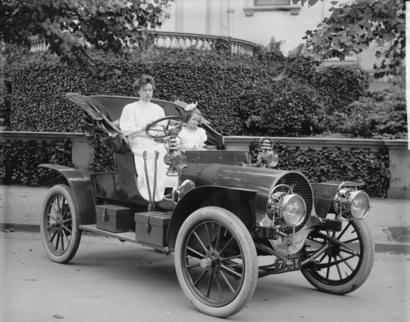
\includegraphics[width=\linewidth]{sample-franklin}
  \caption{1907 Franklin Model D roadster. Photograph by Harris \&
    Ewing, Inc. [Public domain], via Wikimedia
    Commons. (\url{https://goo.gl/VLCRBB}).}
  \Description{A woman and a girl in white dresses sit in an open car.}
\end{figure}

Ihre Zahlen sollten eine Beschriftung enthalten, die die Figur dem Leser beschreibt.

Bildunterschriften werden die Figur platziert.

Jede Figur sollte auch eine Figur Beschreibung haben, es sei denn, es ist rein dekorativ. Diese Beschreibungen vermitteln, was im Bild zu jemandem, der es nicht sehen kann. Sie werden auch von Suchmaschinen-Crawler für die Indizierung von Bildern verwendet, und wenn Bilder nicht geladen werden können.

Für Zahlen, die wichtige und komplexe neue Informationen vermitteln, ist eine kurze Textbeschreibung möglicherweise nicht ausreichend. Komplexere alternative Beschreibungen können in einem Anhang platziert und in einer kurzen Abbildungsbeschreibung referenziert werden. Geben Sie z.B. eine Datentabelle an, die die Informationen in einem Balkendiagramm erfasst, oder eine strukturierte Liste, die einen Graphen darstellt. Weitere Informationen darüber, wie man Figurenbeschreibungen am besten schreibt und warum dies so wichtig ist, finden Sie unter \url{https://www.acm.org/publications/taps/describing-figures/}.

{\itshape unten}{\bfseries Bildbeschreibungen sollten die Bildunterschrift nicht wiederholen – ihr Zweck ist es, wichtige Informationen zu erfassen, die nicht bereits in der Bildunterschrift oder dem Haupttext des Papiers enthalten sind.}\subsection{Die Teaserfigur}

Eine "Teaser-Figur" ist ein Bild oder ein Satz von Bildern in einer Figur, die nach allen Autor- und Zugehörigkeitsinformationen platziert werden, und vor dem Körper des Artikels, über die Seite. Wenn Sie eine solche Figur in Ihrem Artikel haben möchten, legen Sie den Befehl unmittelbar vor dem Befehl \verb|\maketitle|:
\begin{verbatim}
  \begin{teaserfigure}
    \includegraphics[width=\textwidth]{sampleteaser}
    \caption{figure caption}
    \Description{figure description}
  \end{teaserfigure}
\end{verbatim}

\section{Zitate und Bibliographien}

Die Verwendung von \BibTeX für die Vorbereitung und Formatierung der eigenen Referenzen wird dringend empfohlen. Die Namen der Autoren sollten vollständig sein — verwenden Sie vollständige Vornamen (-) Donald E. Knuth-) nicht Initialen (-) und die wichtigsten Merkmale einer Referenz sollten enthalten sein: Titel, Jahr, Volumen, Anzahl, Seiten, Artikel DOI, etc.

Die Bibliographie ist in Ihrem Quelldokument mit diesen beiden Befehlen enthalten, die kurz vor dem Befehl \verb|\end{document}| platziert sind:
\begin{verbatim}
  \bibliographystyle{ACM-Reference-Format}
  \bibliography{bibfile}
\end{verbatim}
Hier ist der Name der \BibTeX-Datei, ohne das Suffix der \BibTeX-Datei.

Verweise und Verweise sind standardmäßig nummeriert. Eine kleine Anzahl von ACM-Publikationen haben Zitate und Verweise, die im Stil des Autorsformatiert sind; für diese Ausnahmen geben Sie bitte diesen Befehl in die (vor dem Befehl "\verb|\begin{document}|") Ihrer \LaTeX-Quelle ein:
{Nr. 1_ Präambel}\begin{verbatim}
  \citestyle{acmauthoryear}
\end{verbatim}

  A couple of preprints \cite{Bornmann2019,
    AnzarootPBM14}cass #17, a master document \cite{Smith10}, a couple of the art_16_cass #17, a master document \cite{VanGundy07}, a enumerated journal article \cite{Cohen07}, a reference to an whole issue \cite{JCohen96}, a monography (whole book) \cite{Kosiur01}, a monography/whole book in a series (siehe 2a in spec. document) \cite{Harel79}, a divisible book as anthology or compilation \cite{Editor00} gefolgt von dem gleichen Beispiel, aber wir geben die Serie nur aus, wenn die Nummer \cite{Editor00a} (so Editor00a's Serie sollte NICHT vorhanden sein, da es keine Vol. Nr.), ein Kapitel in einem divisiblen Buch \cite{Spector90}, ein Kapitel in einem divisiblen Buch in einer Serie \cite{Douglass98}, ein mehrbändiges Werk als Buch \cite{Knuth97}, ein paar Artikel in einem Verfahren (von einer Konferenz, Symposium, Workshop zum Beispiel) \cite{Andler79, Hagerup1993}

\section{Danksagungen}

Die Identifizierung von Finanzierungsquellen und andere Unterstützung, und dank der Einzelpersonen und Gruppen, die in der Forschung und der Vorbereitung der Arbeit unterstützt werden, sollte in eine Anerkennung Abschnitt, der kurz vor dem Referenz-Abschnitt in Ihrem Dokument platziert werden.

Dieser Abschnitt hat eine besondere Umgebung:
\begin{verbatim}
  \begin{acks}
  ...
  \end{acks}
\end{verbatim}
so dass die darin enthaltenen Informationen während der Extraktionsphase der Artikel-Metadaten leichter erfasst werden können und um die Konsistenz in der Schreibweise der Überschrift des Abschnitts zu gewährleisten.

Autoren sollten diesen Abschnitt nicht als nummeriert oder unnummeriert vorbereiten; bitte verwenden Sie die Umgebung.

{\verb|\section|}{\verb|acks|}\section{Anlagen}

Wenn deine Arbeit einen Anhang benötigt, füge ihn vor dem Befehl "\verb|\end{document}|" am Ende deines Quelldokuments hinzu.

Starten Sie den Anhang mit dem Befehl »\verb|appendix|«:
\begin{verbatim}
  \appendix
\end{verbatim}
und beachten Sie, dass in der Anlage, Abschnitte sind Buchstaben, nicht nummeriert. Dieses Dokument hat zwei Anhänge, die den Abschnitt und Unterabschnitt Identifizierungsmethode.

\section{Mehrsprachige Arbeiten}

Papiere können in anderen Sprachen als Englisch geschrieben werden oder Titel, Untertitel, Schlüsselwörter und Abstracts in verschiedenen Sprachen enthalten (in der Regel sollte ein Papier in einer anderen Sprache als Englisch einen englischen Titel und einen englischen Abstract enthalten). Verwenden Sie \verb|language=...| für jede Sprache im Papier verwendet. Die letzte Sprache angegeben ist die Hauptsprache des Papiers. Zum Beispiel kann ein französisches Papier mit zusätzlichen Titeln und Abstracts in Englisch und Deutsch mit dem folgenden Befehl beginnen
\begin{verbatim}
\documentclass[sigconf, language=english, language=german,
               language=french]{acmart}
\end{verbatim}

Titel, Untertitel, Schlüsselwörter und Abstract werden in der Hauptsprache des Papiers eingegeben. Die Befehle \verb|\translatedXXX|, \verb|XXX| begin title, subtitle und keywords können verwendet werden, um diese Elemente in den anderen Sprachen zu setzen. Die Umgebung \verb|translatedabstract| wird verwendet, um die Übersetzung des Abstracts einzustellen. Diese Befehle und Umgebung haben ein obligatorisches erstes Argument: die Sprache des zweiten Arguments. Siehe \verb|sample-sigconf-i13n.tex| Datei für Beispiele ihrer Verwendung.

\section{SIGCHI Extended Abstracts}

Der Schablone-Stil (verfügbar nur in \LaTeX und nicht in Word) erzeugt einen formatierten Landscape-Orientierung-Artikel mit einem breiten linken Rand. Drei Umgebungen stehen für den Schablone-Stil zur Verfügung und erzeugen formatierte Ausgabe im Rand:
\begin{description}
\item[\texttt{sidebar}:]  Legen Sie formatierten Text in den Rand.
\item[\texttt{marginfigure}:] Legen Sie eine Figur in den Rand.
\item[\texttt{margintable}:] Legen Sie eine Tabelle in den Rand.
\end{description}

%%
%% The acknowledgments section is defined using the "acks" environment
%% (and NOT an unnumbered section). This ensures the proper
%% identification of the section in the article metadata, and the
%% consistent spelling of the heading.
\begin{acks}
Für Robert, für die Bagels und erklären CMYK und Farbräume.
\end{acks}

%%
%% The next two lines define the bibliography style to be used, and
%% the bibliography file.
\bibliographystyle{ACM-Reference-Format}
\bibliography{sample-base}

%%
%% If your work has an appendix, this is the place to put it.
\appendix

\section{Forschungsmethoden}

\subsection{Erster Teil}

Lorem ipsum dolor sit amet, consectetur adipiscing elit. Morbi malesuada, quam in pulvinar varius, metus nunc fermentum urna, id sollicitudin purus odio sit amet enim. Aliquam ullamcorper eu ipsum vel mollis. Curabitur quis dictum nisl. Phasellus vel semper risus, et lacinia dolor. Integer ultricies commodo sem nec semper.

\subsection{Zweiter Teil}

Etiam commodo feugiat nisl pulvinar pellentesque. Etiam auctor sodales ligula, non varius nibh pulvinar semper. Suspendisse nec lectus non ipsum convallis congue hendrerit vitae sapien. Donec at laoreet eros. Vivamus non purus placerat, scelerisque diam eu, cursus ante. Etiam aliquam tortor auctor efficitur mattis.

\section{Online-Ressourcen}

Nam id fermentum dui. Suspendisse sagittis tortor a nulla mollis, in pulvinar ex pretium. Sed interdum orci quis metus euismod, et sagittis enim maximus. Vestibulum gravida massa ut felis suscipit congue. Quisque mattis elit a risus ultrices commodo venenatis eget dui. Etiam sagittis eleifend elementum.

Nam interdum magna at lectus dignissim, ac dignissim lorem rhoncus. Maecenas eu arcu ac neque placerat aliquam. Nunc pulvinar massa et mattis lacinia.

\end{document}
\endinput%%
%% End of file `sample-manuscript.tex'.
